\documentclass{article}
\usepackage{graphicx}
\usepackage[utf8]{inputenc}
\usepackage[T1]{fontenc}
\usepackage{fouriernc}
\usepackage[margin=1in]{geometry}
\usepackage{amsmath}

\begin{document}

\begin{titlepage}
	\centering 
	\scshape
	\vspace*{\baselineskip}
	\rule{\textwidth}{1.6pt}\vspace*{-\baselineskip}\vspace*{2pt}
	\rule{\textwidth}{0.4pt} 
	\vspace{0.75\baselineskip}
	
	{\Large CS 374 : Computational and Numerical Methods \\\vspace{0.75\baselineskip} Assignment 1 - Set 2}
	\vspace{0.75\baselineskip}
	
	\rule{\textwidth}{0.4pt}\vspace*{-\baselineskip}\vspace{3.2pt} 
	\rule{\textwidth}{1.6pt}
	
	\vspace{2\baselineskip}  
	%Title
	
	\vspace*{3\baselineskip}
	%Subtitle
	
	\vspace{0.5\baselineskip} %originally 0.5
	
	{\scshape\large Purvil Mehta (201701073) \\ Bhargey Mehta (201701074) \\} 
	
	\vspace{1\baselineskip} 
	
	\textit{Dhirubhai Ambani Institute of Information and Communication Technology \\ Gandhinagar\\} 
	\vspace*{2\baselineskip}
	\today


\end{titlepage}

\newpage
\tableofcontents
\newpage
\section{Approximation of functions using Taylor Polynomials}
\par Consider the following functions:
\begin{itemize}
    \item $y = e^x$
    \item $y = \ln{x}$
    \item $y = \sin{x}$
    \item $y = \cos{x}$
\end{itemize}
Produce the first, the second and the third-degree Taylor polynomials for each of the foregoing functions, using a=1 as the point of approximation for $\ln{x}$ and a=0 for the rest.In a suitably chosen neighborhood of a, follow how the accuracy of a Taylor polynomial improves with its increasing degree. For this you will have to estimate the difference between f(x) and its Taylor polynomials in a code. Present your result  for each function along with its Taylor polynomials of all 3 degrees.
\subsection{Approximation for $e^{x}$}
\subsubsection{Plot}
\begin{figure}[!h]
    \centering
    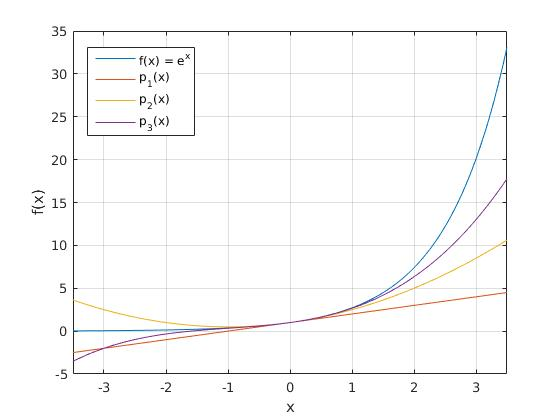
\includegraphics[scale = 0.4]{19}
    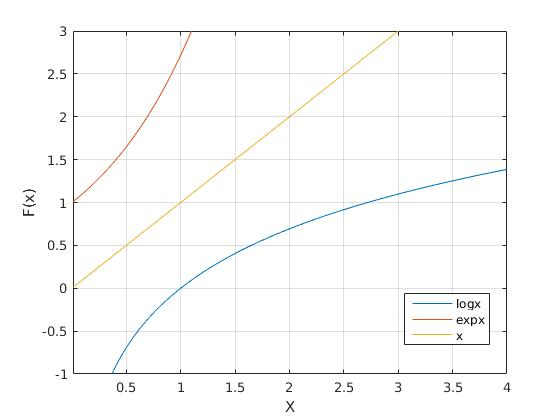
\includegraphics[scale = 0.4]{2}
    \caption{Behaviour of Different Order polynomial}
    \label{fig:ques1}
\end{figure}

\subsubsection{Observations}
\begin{itemize}
    
    \item Using Taylor Series which is given by \begin{equation} \label{eqn:taylor}f(x) = f(x_{0}) + \frac{ f'(x_{0})(x - x_{0})}{1!} + \frac{f''(x_0)(x - x_0)^2}{2!} + ...\end{equation}
    We approximate the function till the third order of the series around $a=0$ .
    
    \item As we observed that the even order polynomial rises up in the positive direction as $x\to -\infty$ and exactly this kind of graph we got in the figure 1. \textbf{As \textbf{$p_2(x)$} in the graph lies above the actual graph}. 
    
    \item In the case of odd order polynomial equation which goes to $-\infty$ as $x\to-\infty$ and that is why we got $p_1(x)$ and $p_3(x)$ which goes to $-\infty$ shown in the figure.\textbf{These polynomial lies under the actual function curve.}
    
    \item \textbf{The positive side of the graph, sign will not affect the Taylor polynomial and all the Taylor polynomials lies below the actual function as we have approximated the function.}
    
    
\end{itemize}

\newpage
\subsection{Approximation for $\ln{x}$}
\subsubsection{Plot}
\begin{figure}[!h]
    \centering
    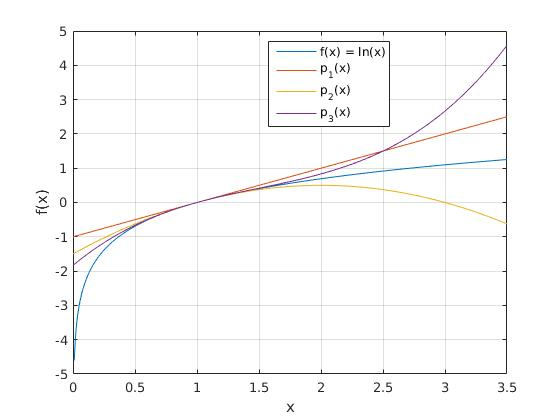
\includegraphics[scale = 0.4]{20}
    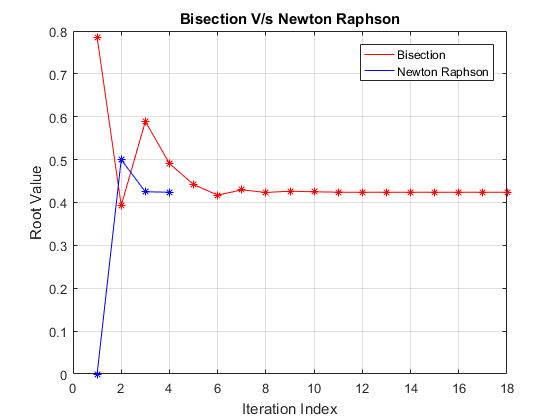
\includegraphics[scale = 0.4]{4}
    \caption{Behaviour of Different Order polynomial}
    \label{fig:ques2}
\end{figure}

\subsubsection{Observations}
\begin{itemize}
    
    \item Using Taylor Series which is given by equation \ref{eqn:taylor}, we approximate the function till the third order of the series around $a = 1$ as it is given in the question.
    
    
    \item As we observed that the value of even order polynomial decreases or goes to $\to-\infty$  as the value of x increases in the positive direction.Thus for smaller value of x even order polynomial behaves like $\ln{x}$. But for large value of x, the higher even order with negative sign brigs the function down in the negative direction.  \textbf{As \textbf{$p_2(x)$} in the graph lies below the actual graph}. 
    
    \item In the case of odd order polynomial equation which goes to $\infty$ as $x\to\infty$ and that is why we got $p_1(x)$ and $p_3(x)$ which goes to $\infty$ shown in the figure.\textbf{These polynomial lies above the actual function curve.}
    
    \item \textbf{In between [0-1], value of x will not affect the Taylor polynomial and all the Taylor polynomials lies above the actual function as we have approximated the function.}
    
    \item As we consider more and more degree in the Taylor Polynomial Series, we get closer and closer graph compared to the actual function.
    
    
\end{itemize}
\newpage
\subsection{Approximation for $\sin{x}$}
\subsubsection{Plot}
\begin{figure}[!h]
    \centering
    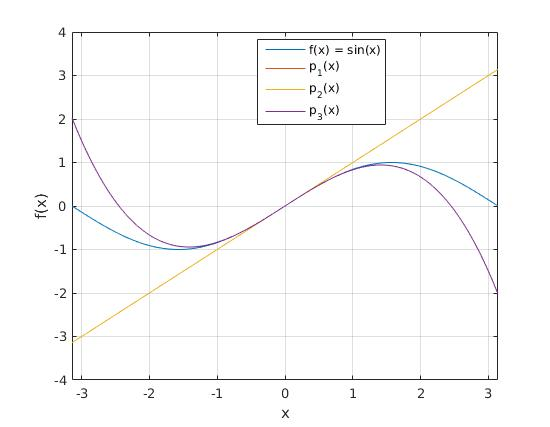
\includegraphics[scale = 0.4]{21}
    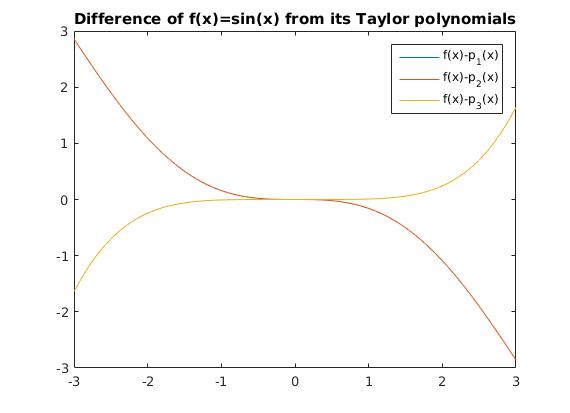
\includegraphics[scale = 0.4]{6}
    \caption{Behaviour of Different Order polynomial}
    \label{fig:ques3}
\end{figure}

\subsubsection{Observations}
\begin{itemize}
    
    \item Using Taylor Series which is given by equation \ref{eqn:taylor}, we approximate the function till the third order of the series around $a = 0$ as it is given in the question.
    
    
    \item For any value of x, the first order Taylor polynomial which is nothing but a straight line does not have any turning point and thus form small value of x it shows the correct output but shows incorrect output for large value of x. 
    
    \item For small value of x eg.[0-1], the third order Taylor polynomial will behave like straight line as we neglect the $x^3$ part of the polynomial.But as the value for the x increases, the higher order term with the minus sign brings the function down toward $-\infty$. In the negative direction, since higher order of the function is three with minus sign takes the function up in the $+\infty$.
    
    Since the first derivative of the $p_{3}(x)$ is $p_3'(x) =  1 - \frac{x^2}{2}$ which has two turning points at $x = \pm\sqrt{2}$.Also the second derivative of $p_{3}(x)$ is $p_3''(x) =  -x$. Thus function has minima at $x =\sqrt{2}$ and maxima at $x =-\sqrt{2}$. And thus more and more degree of the Taylor polynomial takes us more closer to the actual function.
    
    Since $p_3(x)$ has root at $ x = \sqrt{6}$, the decreasing rate of the function is more than the actual function. 
\newpage    
    
\end{itemize}
\subsection{Approximation for $\cos{x}$}
\subsubsection{Plot}
\begin{figure}[!h]
    \centering
    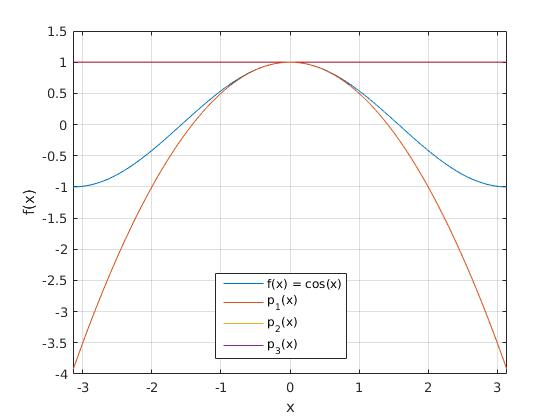
\includegraphics[scale = 0.4]{22}
    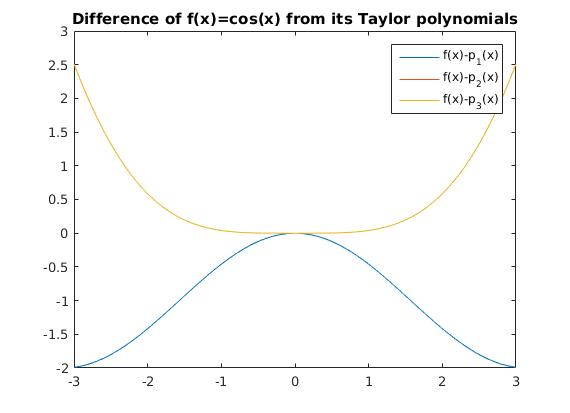
\includegraphics[scale = 0.4]{8}
    \caption{Behaviour of Different Order polynomial}
    \label{fig:ques4}
\end{figure}

\subsubsection{Observations}
\begin{itemize}
    
    \item Using Taylor Series which is given by equation \ref{eqn:taylor}, we approximate the function till the third order of the series around $a = 0$ as it is given in the question.
    
    
    \item For any value of x, the first order Taylor polynomial which is nothing but a constant line does not have any turning point and thus form small value of x it shows the correct output but shows incorrect output for large value of x. 
    
    \item For small value of x eg.[$-\frac{\pi}{2}$-$\frac{\pi}{2}$], the second order Taylor polynomial will behave like cosine function as we neglect the $x^2$ part of the polynomial.But as the value for the x increases, the higher order term with the minus sign brings the function down toward $-\infty$. In the negative direction, since higher order of the function is two with minus sign will not affect the function and takes down in the $-\infty$.
    
    Since the first derivative of the $p_{2}(x)$ is $p_2'(x) =  -x$ which has only one turning point at $x = 0$.Also the second derivative of $p_{2}(x)$ is $p_2''(x) =  -1$. Thus function has maxima at $x = 0$. And thus for some values eg. [$-\frac{\pi}{2}$-$\frac{\pi}{2}$] function behaves like cosine function but the function goes to $-\infty$ for increasing values of x in positive as well as negative direction.
    
    Since $p_3(x)$ has root at $ x = \pm\sqrt{2} \approx \pm1.41$, the decreasing rate of the function is more than the actual function. 
    
    
\end{itemize}
\end{document}